%---------------------------------------------------------------------
\chapter{Experimentation}
\label{ch:exp}
%---------------------------------------------------------------------

\section{Hypothesis}
The design decision that the experiment informs is whether to let the model choose each check (V2) or to run a
fixed sequence of checks and let the model only assess (V1). Adaptive choice is the characteristic agentic
behaviour, and it costs a planning call per check. The hypothesis, stated before any held-out run, is the
following.

\begin{quote}
\textbf{H1.} On the same dossiers, with the same tools, corpus and budget, V2 attains a higher supported
case-success rate than V1 at a lower or comparable cost in model calls.
\end{quote}

\textbf{H1 is a hypothesis and not a result.} The development runs give a reason to doubt it, because V2 was not
more successful than V1 on the development dossiers (Section~\ref{sec:devquality}), and a negative outcome is
a valid result that will be reported as such. A secondary hypothesis is that V2 uses fewer model calls than
V1, which the development runs support: 1.8 calls against 5.5 on average.

\section{Experimental Setup}
\label{sec:expsetup}
\begin{itemize}[itemsep=2pt]
\item \textbf{Cases.} The 24 held-out dossiers of \code{pilot-0.1}, of which two are expected preflight stops.
\item \textbf{Variants.} V1 and V2 with the real model; V0 and SC as controls (Table~\ref{tab:variantdef}).
\item \textbf{Fixed factors.} Model and weights revision, prompt version, tools, corpus, index, calculation
      profile and budget are the same for both variants and are pinned in a freeze record that is verified
      before a held-out run is allowed.
\item \textbf{Order and repeats.} The order of V1 and V2 alternates by case. Each pair is repeated $R$ times
      because greedy decoding on a GPU is not guaranteed to repeat exactly. The value of $R$ is decided together
      with the freeze, before any held-out run, and a value of $R=3$ is proposed \pendingtext{decision of $R$}.
\item \textbf{Analysis.} A paired case-level bootstrap with a fixed seed resamples cases with all of their
      repeats; repeats are not independent samples, so per-trial means and the share of cases in which all repeats
      succeed are both reported.
\item \textbf{Stopping rules.} A night stops after seven hours, two million tokens, three consecutive
      infrastructure failures or when a kill-switch file exists. Unfinished trials are counted as not run.
\end{itemize}
Held-out runs are launched only with a freeze record that includes the real model, names the protocol by
digest and names the held-out location. Development is the default, and a fixture dry run cannot use the
held-out flag.

\section{Development Experiments with the Prompt}
\label{sec:promptdev}
Before the held-out run the prompt was tuned on development dossiers only. The 24 development dossiers were split
by a fixed digest, without using any result, into a tuning set of 16 and a checking set of 8. The prompt was
changed only on the tuning set, each change was a new version, and the checking set was run once at the end and was
not used to tune. The held-out dossiers were never opened. Table~\ref{tab:promptdev} records every version. The
versions v5 and v6 were evaluated on all 24 development dossiers, and v7 to v9 on the tuning set of 16.

\begin{table}[H]
\centering
\caption{Prompt versions and what was observed on development dossiers}
\label{tab:promptdev}
\small
\begin{tabularx}{\linewidth}{@{}l p{3.4cm} X@{}}
\toprule
\textbf{Version} & \textbf{Change} & \textbf{Observed} \\ \midrule
v5 & Baseline. & 29 of 48 trials not failed (V1 21 of 24, V2 8 of 24). Failures from invented observation ids, invalid abstention reasons and invalid issue types. Schema-valid at most 83\% of calls. \\
v6 & Rules for the three v5 failure causes. & 40 of 48 not failed (V1 24 of 24, V2 16 of 24). All 8 V2 failures were invented observation ids. \\
v7 & Refused-action repair added to the runner. & 32 of 32 not failed; 100\% schema-valid; the model made no finding proposal in any run. \\
v8 & Defined what counts as a problem; removed a copied refutation example. & 32 of 32 not failed; 40 schema-invalid V1 attempts needed a retry because the model placed the proposal at the top level of its reply; still no accepted proposal; V1 mean wall time rose to 208\,s. \\
v9 & Example proposal shown nested under its key. & 32 of 32 not failed; no retries; V1 made 13 proposals and 1 was accepted; V1 mean wall time 141\,s. \\
\bottomrule
\end{tabularx}
\end{table}

\begin{figure}[H]
\centering
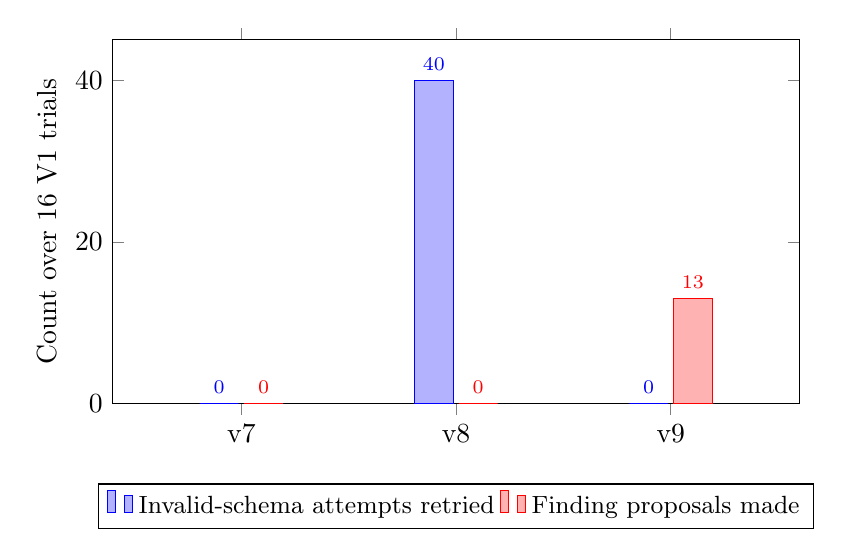
\begin{tikzpicture}
\begin{axis}[
  ybar, bar width=14pt, width=0.85\linewidth, height=6.2cm,
  symbolic x coords={v7,v8,v9}, xtick=data,
  ylabel={Count over 16 V1 trials},
  ymin=0, ymax=45, legend style={at={(0.5,-0.22)},anchor=north,legend columns=-1,font=\small},
  nodes near coords, every node near coord/.append style={font=\scriptsize},
  enlarge x limits=0.3]
\addplot coordinates {(v7,0) (v8,40) (v9,0)};
\addplot coordinates {(v7,0) (v8,0) (v9,13)};
\legend{Invalid-schema attempts retried, Finding proposals made}
\end{axis}
\end{tikzpicture}
\caption{Effect of the prompt version on V1 in the tuning set. The version v8 moved the model from never
proposing to proposing in a malformed structure, and v9 fixed the structure.}
\label{fig:promptdev}
\end{figure}

Three points follow. First, each change corrected the failure it targeted, and the failure moved to the next
layer, from invented identifiers to a model that never proposes, and then to a model that proposes in
words the gate refuses. Second, none of the changes increased the supported case-success rate, which stayed
at 2 of 16 for both variants in v7, v8 and v9. Third, the checking set, which was run once after tuning ended, also had
no failed run (16 of 16 not failed, 100\% schema-valid per call); it is a small set from the same generator, so it
is a weak check on overfitting and not a proof against it.

\section{Results}
\pending{The held-out comparison has not been run, so there is no result to report here. When it exists, this
section will give, from the generated tables only: the success rate of V0, SC, V1 and V2 with intervals, the
paired difference between V2 and V1 with and without the two preflight cases, the efficiency in calls, tokens and
time, and the agreement of repeats. A plot of success against model calls per variant is planned.}

\section{Discussion and Decision}
\pending{The decision on whether adaptive investigation is worth its cost depends on the held-out result and
is not made in this report draft. The development evidence points to two conclusions that will be checked:
the adaptive variant is cheaper in calls, and neither variant yet adds findings beyond the deterministic checks.
If the held-out result agrees, the decision will state that on this setup the fixed variant is not worse, and
the discussion will say so.}
